\documentclass[review,12pt]{elsarticle}

\journal{Journal of Computational Physics}

\usepackage{amsmath,amssymb,amsfonts}
\usepackage{graphicx}
\usepackage{booktabs}
\usepackage{hyperref}

\begin{document}

\begin{frontmatter}

\title{Residual multi-fidelity neural network correction of a Sutherland-type $\eta\to D$ map for Al-dominated liquid alloys}

\author[a]{Tina Young}
\ead{TBD}

\address[a]{Affiliation TBD}

\begin{abstract}
Liquid diffusivity $D$ in multicomponent melts is scarce relative to viscosity $\eta$, yet Stokes--Einstein / Sutherland-type relations only partially map $\eta$ to $D$. Prior melt practice largely stops at analytic Stokes--Einstein / Sutherland maps or single-fidelity fits that neither treat LF physics and HF experiments as distinct fidelities nor separate within-composition temperature generalization from composition leave-out. We couple a modified Sutherland low-fidelity (LF) prior---built from measured or recommended $\eta$~\cite{assael2006,schick2012,tang2015}---to a residual multi-fidelity neural network (MFNN) in the sense of Lu et al.~\cite{lu2020pnas}, which extends the composite multi-fidelity network of Meng and Karniadakis~\cite{meng2020jcp}, correcting $\log_{10} D_{\mathrm{LF}}$ toward high-fidelity (HF) experimental diffusivities while encoding composition and, where needed, diffusion type. Learning in $\log_{10} D$ enforces positivity and corresponds to a multiplicative correction in linear $D$. The scope is primarily Al--Cu with auxiliary ternary context under honest $\eta$ pairing (not cross-system LOGO). Under a within-composition temperature hold-out (Protocol W; five seeds; $n_{\mathrm{test}}=15$), the residual MFNN attains MAPE $26.18\pm 1.33\%$ and Factor2 $0.96\pm 0.033$, improving on HF-only in mean accuracy ($30.98\pm 4.43\%$) and seed-to-seed MAPE standard deviation ($\sim$70\% reduction, $4.43\to 1.33$), and far exceeding LF-only ($\sim$109.6\%). Al--Cu leave-one-composition-out with \texttt{diff\_type} splitting and one-hot features yields overall MAPE $39.43\pm 39.71\%$ and is reported only as a cautionary check: Al80Cu20 interdiffusivity folds recover, while tracer hold-outs remain failed, so composition extrapolation stays bounded.
\end{abstract}

\begin{highlights}
\item Residual MFNN corrects a Sutherland $\eta\to D$ prior for Al-dominated melts
\item Protocol W: MFNN MAPE 26.18$\pm$1.33\%, Factor2 0.96$\pm$0.033; $\sim$70\% MAPE-std cut vs HF-only
\item Honest $\eta$ pairing; no Kozlov silent fill; densified Arrhenius labeled
\item Tracer/inter label split and one-hot improve Al--Cu LOGO diagnosis
\item Composition leave-out limited by sparse tracer HF neighborhoods
\end{highlights}

\begin{keyword}
Multi-fidelity neural network \sep Liquid diffusivity \sep Viscosity \sep Stokes--Einstein--Sutherland \sep Aluminum alloys \sep Leave-one-composition-out
\end{keyword}

\end{frontmatter}

%% ============================================================
\section{Introduction}
\label{sec:intro}

Transport coefficients of liquid alloys control solidification microstructure, impurity redistribution, and process models in casting and additive manufacturing. Among them, self- and interdiffusivities $D(T,\{x_i\})$ are experimentally expensive: capillary, shear-cell, and quasielastic neutron or X-ray methods yield sparse tables that mix tracer, interdiffusivity, and impurity definitions. Viscosity $\eta(T,\{x_i\})$, by contrast, is more routinely measured or recommended for pure metals and several binaries (e.g.\ Assael compilations for Al~\cite{assael2006}; Schick et al.\ for Al--Cu~\cite{schick2012}). Classical Stokes--Einstein and Sutherland links therefore remain a natural bridge from $\eta$ to $D$, and melt-specific modifications with temperature-dependent effective radii have been developed for Al-based liquids~\cite{tang2015,chen2014}. In practice, however, a pure physics map is only a first-order prior: slip/stick assumptions, radius choices, and the mismatch between tracer and chemical diffusivities leave systematic residuals against HF labels.

Data-driven multi-fidelity learning offers a structured way to keep that physics prior while learning corrections from scarce HF data. Meng and Karniadakis~\cite{meng2020jcp} introduced a composite neural network that learns from multi-fidelity data by coupling a low-fidelity network to linear and nonlinear high-fidelity branches. Lu et al.~\cite{lu2020pnas} extended that composite construction with a residual multi-fidelity neural network, composing a linear map of low-fidelity outputs with a nonlinear residual. We adopt the residual MFNN formulation of Lu et al.~\cite{lu2020pnas} for $\eta\to D$ regression, enabling high-fidelity calibration with improved stability under scarce expensive labels. The model is a residual MFNN in the Lu/Meng sense~\cite{lu2020pnas,meng2020jcp}: scientific content enters through the LF Sutherland $\eta\to D$ channel, not as a PDE-residual PINN/PPINN~\cite{karniadakis2021}. Prior $\eta\to D$ practice in melts has largely stopped at analytic Stokes--Einstein / Sutherland maps or simple regressions that do not (i) treat LF physics and HF experiments as distinct fidelities, (ii) evaluate within-composition temperature generalization separately from composition leave-out, or (iii) diagnose tracer versus interdiffusivity label conflicts under honest viscosity pairing.

This work addresses that gap for Al-dominated melt alloys. Our contributions are:
\begin{enumerate}
\item \textbf{Residual MFNN for $\eta\to D$.} We cast prediction as multi-fidelity regression on $\log_{10} D$: a Chen/Tang-style Sutherland LF channel~\cite{tang2015,chen2014} supplies $D_{\mathrm{LF}}$ from honest $\eta$, and a Lu-style residual MFNN~\cite{lu2020pnas} (extending Meng and Karniadakis~\cite{meng2020jcp}) corrects toward HF experimental $D$, with composition features and optional \texttt{diff\_type} one-hot encoding.

\item \textbf{Honest provenance.} Rows without usable experimental or Assael/Schick-class $\eta$~\cite{assael2006,schick2012} are dropped; Kozlov alloy viscosity is never used as a silent HF $\eta$ fill; densified Zhang Arrhenius grids~\cite{zhang2010prl} are labeled as such, not as independent experiments.

\item \textbf{Protocol separation (W / G / LOGO).} Within-composition temperature splits (protocol W) are the primary claim; random between-group splits (G) are cautionary only; Al--Cu leave-one-composition-out (LOGO) is reported as internal composition extrapolation, not cross-system generalization.

\item \textbf{Tracer / interdiffusivity diagnosis.} Mixed composition groups that conflate Cu-tracer and interdiffusivity at nearly the same $T$ are split and analyzed; neighborhood sparsity of tracer HF---not the residual architecture alone---explains hard LOGO folds and the failure of separate tracer/inter models to beat a joint model with one-hot \texttt{diff\_type}.
\end{enumerate}

Together, Methods and Results below show stable within-group gains of MFNN over HF-only and LF-only baselines, while Limitations state explicitly what we do not claim.

%% ============================================================
\section{Methods}
\label{sec:methods}

\subsection{Problem formulation}
\label{sec:problem}

We aim to predict liquid-alloy diffusivity $D$ from measured viscosity $\eta$, temperature $T$, and composition $\{x_i\}$. Experimental diffusivities for multicomponent melts are sparse and of mixed physical type (tracer vs interdiffusivity), whereas viscosity data---and viscosity--diffusivity relations of Stokes--Einstein / Sutherland type---are comparatively more available. We therefore cast prediction as a multi-fidelity regression problem: a low-fidelity (LF) physics map $\eta \mapsto D_{\mathrm{LF}}$ supplies a continuous prior, and a residual multi-fidelity neural network (MFNN) corrects that prior toward high-fidelity (HF) experimental $D$ labels.

All supervised targets are $\log_{10} D$ (with $D$ in $\mathrm{m}^{2}\,\mathrm{s}^{-1}$). Reported MAPE and Factor2 are evaluated after transforming predictions back to linear $D$.

\subsection{Data and provenance}
\label{sec:data}

\textbf{Sources.} HF diffusivities are compiled from published melt measurements, with Al--Cu the dominant chemistry~\cite{chen2014,zhang2010prl,geng2014}. Viscosities paired to HF rows use measured or recommended correlations where available: Assael et al.~\cite{assael2006} for pure Al $\eta$, Schick et al.~\cite{schick2012} for Al--Cu $\eta$, and Tang et al.~\cite{tang2015} for Al--Mg--Si context. In sample composition the usable HF table is Al--Cu--dominated: Al--Mg--Si and Al--Ce--Ni appear only as thinner background coverage, enter training solely where honest $\eta$ pairing exists, and remain insufficient for cross-system leave-one-out (LOGO).

\textbf{Honesty rules.} Rows lacking a usable experimental (or Assael/Schick-class) $\eta$ are dropped. Kozlov alloy viscosity is never used as a silent HF $\eta$ fill. Where Zhang (and related) Arrhenius parameters are densified onto a temperature grid~\cite{zhang2010prl}, those grid points are treated as densified Arrhenius samples, not as independent experiments.

\textbf{Composition groups and diffusion type.} Each row carries a composition-group label \texttt{comp\_group} (e.g.\ Al80Cu20) and a diffusion-type label \texttt{diff\_type} (tracer, interdiffusivity / inter, impurity, etc.). A diagnostic on Al80Cu20 showed that a single \texttt{comp\_group} mixed Cu-tracer HF values ($\sim 2.3$--$4.9\times 10^{-9}\,\mathrm{m}^{2}\,\mathrm{s}^{-1}$) with interdiffusivity values ($\sim 7$--$8.9\times 10^{-9}$) at nearly the same $T$, a $\sim 3\times$ label conflict, while features lacked \texttt{diff\_type} and the failure was not out-of-distribution in $x_{\mathrm{Cu}}$ or $T$; Schick $\eta$ pairing was sound. We therefore split mixed groups into \texttt{\_tracer} and \texttt{\_inter} subgroups for evaluation folds, and optionally encode \texttt{diff\_type} as a one-hot feature (Sec.~\ref{sec:features}).

Training uses the $\eta$-paired table loaded from \texttt{data/melt\_diffusion\_data.csv} (compiled LF and HF rows; rows without usable $\eta$ are dropped per the honesty rules above). Evaluations below report the exact test sizes used ($n_{\mathrm{test}}=15$ for protocol W; 11 then 13 Al--Cu LOGO folds after the \texttt{diff\_type} split).

\subsection{Low-fidelity physics mapping}
\label{sec:lf}

Given $\eta(T,\{x_i\})$ and an effective hard-sphere radius for the diffuser, LF diffusivity targets are obtained from a modified Sutherland / Stokes--Einstein relation in the sense of Chen et al.~\cite{chen2014}, with temperature-dependent radii consistent with that framework and with Tang et al.~\cite{tang2015} for multicomponent Al melts. Symbolically,
\begin{equation}
\label{eq:sutherland}
D_{\mathrm{LF}} \propto \frac{k_{\mathrm{B}} T}{\eta\, r_{\mathrm{eff}}(T)}\times \text{(slip/stick correction)},
\end{equation}
and $y_{\mathrm{L}}=\log_{10} D_{\mathrm{LF}}$ enters the MFNN as the LF channel / LF training targets. The reported \textbf{LF\_only} baseline is \textbf{not} the pure analytic Sutherland map evaluated alone: it is the single-fidelity network $F_{\mathrm{L}}$ trained on those Sutherland-generated $\log_{10} D_{\mathrm{LF}}$ targets across the five seeds (code path: \texttt{pred\_lf\_only = model\_lf(...)}). Seed-to-seed variance of LF\_only is therefore expected.

\subsection{Residual multi-fidelity network}
\label{sec:mfnn}

We adopt the residual multi-fidelity architecture of Lu et al.~\cite{lu2020pnas}, which extends the composite multi-fidelity neural network of Meng and Karniadakis~\cite{meng2020jcp}. An LF network $F_{\mathrm{L}}(\mathbf{x})$ is trained on the Sutherland-generated $\log_{10} D_{\mathrm{LF}}$ targets (Sec.~\ref{sec:lf}). The HF predictor composes a linear map and a nonlinear residual network on the concatenated inputs $[\mathbf{x},\, y_{\mathrm{L}}]$:
\begin{equation}
\label{eq:residual}
\hat{y}_{\mathrm{H}}
=
\alpha_1\,
\bigl(A\,[\mathbf{x},\, y_{\mathrm{L}}]+b\bigr)
+
\alpha_2\,
F_{\mathrm{nl}}(\mathbf{x},\, y_{\mathrm{L}}),
\end{equation}
with learnable mixing weights $\alpha_1,\alpha_2$. Single-fidelity MLPs of matching width/depth trained only on HF labels form the \textbf{HF\_only} baseline; the composite residual model is \textbf{MFNN}. (As in Sec.~\ref{sec:intro}: residual / composite multi-fidelity~\cite{lu2020pnas,meng2020jcp}.)

Fig.~\ref{fig:mfnn} illustrates the MFNN schema used in this work. Fig.~\ref{fig:coverage} summarizes honest $\eta$-paired HF coverage and the Sutherland prior context.

\begin{figure}[t]
\centering
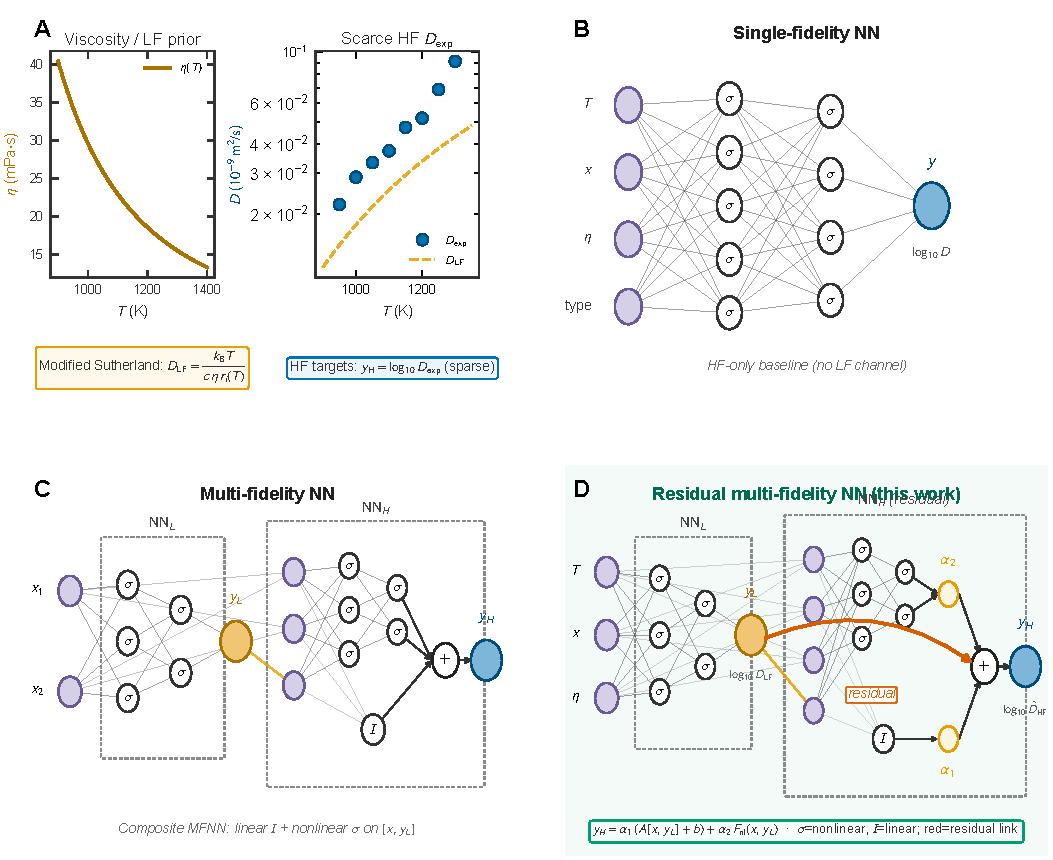
\includegraphics[width=\linewidth]{figures/fig1_mfnn_schema.pdf}
\caption{Schematic of the residual multi-fidelity neural network (MFNN) for predicting high-fidelity liquid diffusivity $D$ from viscosity $\eta$, in the style of Lu et al.\ (PNAS 2020). (A)~Modified Sutherland LF prior $D_{\mathrm{LF}}\propto T/(\eta\,r_i(T))$ versus scarce HF $D_{\mathrm{exp}}$. (B)~Single-fidelity NN (HF-only). (C)~Composite MFNN with linear ($I$) and nonlinear ($\sigma$) branches on $[x,y_L]$. (D)~Residual MFNN used here: $y_H=\alpha_1(A[x,y_L]+b)+\alpha_2 F_{\mathrm{nl}}(x,y_L)$ with learnable $\alpha_1,\alpha_2$ and a residual link from $y_L$; positivity via $\hat{D}=10^{\hat{y}}$. Features $(T,\,x,\,\eta)$ and optional \texttt{diff\_type}.}
\label{fig:mfnn}
\end{figure}

\begin{figure}[t]
\centering
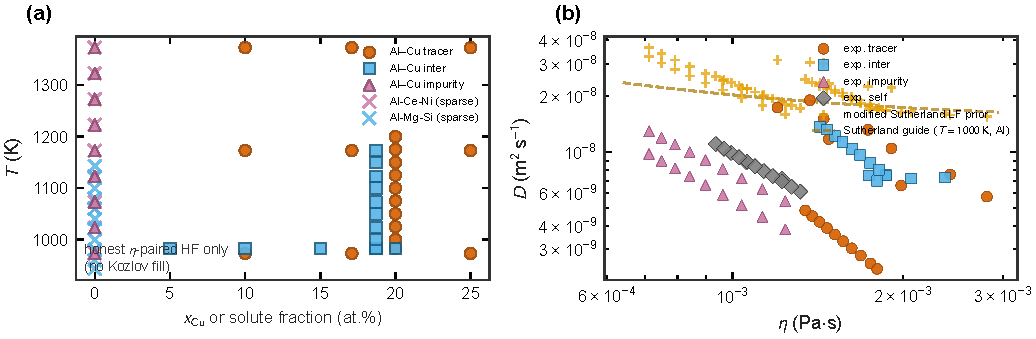
\includegraphics[width=\linewidth]{figures/Fig2_phase_space_coverage.pdf}
\caption{Phase-space coverage and physical context with honest viscosity pairing (no Kozlov fills). (a) HF temperature--composition coverage (Al--Cu by modality; sparse multi-component systems versus non-Al solute fraction). (b) Experimental $D$ versus $\eta$ with modified Sutherland LF prior at the same $(T,\eta)$ and a pure-Al Sutherland guide at $T=1000\,\mathrm{K}$.}
\label{fig:coverage}
\end{figure}

\subsection{Features}
\label{sec:features}

The base continuous feature vector (12 dimensions) is
\begin{equation}
\label{eq:features}
\mathbf{x}
=
\bigl[
T,\;
1000/T,\;
\eta,\;
\log_{10}\eta,\;
x_{\mathrm{Al}},x_{\mathrm{Cu}},x_{\mathrm{Ce}},x_{\mathrm{Ni}},x_{\mathrm{Ag}},x_{\mathrm{Mg}},x_{\mathrm{Si}},\;
r_{\mathrm{diff}}
\bigr],
\end{equation}
with mole fractions zero-padded for absent elements and $r_{\mathrm{diff}}$ the effective diffuser radius (\AA-scale). The Ce/Ni/Ag/Mg/Si coordinates accommodate compiled multicomponent background rows; primary evaluation remains Al--Cu. For stratified LOGO ablations we append a \texttt{diff\_type} one-hot (12 $\to$ 16 features). Continuous features are z-scored using training-set statistics only.

\subsection{Training}
\label{sec:training}

Optimization follows Adam then L-BFGS polishing (MSE on $\log_{10} D$). LF rows supervise $F_{\mathrm{L}}$ on Sutherland-generated $\log_{10} D_{\mathrm{LF}}$ targets; HF rows supervise the residual HF head, with $y_{\mathrm{L}}$ taken from the LF network. Hyperparameters follow \texttt{train.py}: single-fidelity baselines (LF\_only / HF\_only) use width 64, depth 3 tanh MLPs, Adam ($\mathrm{lr}=10^{-3}$, \texttt{adam\_epochs=800}), then L-BFGS ($\mathrm{lr}=0.5$, \texttt{max\_iter=20} per call, $\sim$\texttt{lbfgs\_steps=50}); HF\_only uses \texttt{weight\_decay=}$5\times 10^{-3}$ at the call site (LF\_only default \texttt{weight\_decay=}$10^{-4}$). The residual MFNN uses width 64, Adam ($\mathrm{lr}=10^{-3}$, \texttt{adam\_epochs=1000}, \texttt{weight\_decay=}$10^{-4}$), then L-BFGS ($\mathrm{lr}=0.4$, \texttt{max\_iter=20}, $\sim$\texttt{lbfgs\_steps=40}). Multi-run statistics use seeds $\{0,1,2,42,123\}$.

\subsection{Evaluation protocols W / G / LOGO and metrics}
\label{sec:protocols}

Three protocols are distinguished deliberately:

\begin{table}[t]
\centering
\caption{Protocol definitions for within-composition temperature split (W), random between-group hold-out (G), and leave-one-composition-out (LOGO).}
\label{tab:protocols}
\begin{tabular}{@{}lll@{}}
\toprule
Protocol & Definition & Role in this paper \\
\midrule
\textbf{W} (within-composition $T$-split)
  & Within each \texttt{comp\_group} with sufficient HF $T$ span, hold out a temperature subset ($\sim$25\% of HF, preferring extreme $T$); train on remaining HF + all LF.
  & \textbf{Primary claim} \\
\textbf{G} (random between-group)
  & Seed-dependent hold-out of composition groups.
  & Caution / SI only; not a headline result \\
\textbf{LOGO}
  & Fixed leave-one-\texttt{comp\_group}-out on Al--Cu (11 folds before \texttt{diff\_type} split; 13 after).
  & Composition-extrapolation exploration; stratified by \texttt{diff\_type} \\
\bottomrule
\end{tabular}
\end{table}

\textbf{Metrics.} Mean absolute percentage error (MAPE, \%), Factor2 (fraction of predictions within a factor of two of HF $D$), and $R^{2}$ on $\log_{10} D$ where reported. Multi-seed summaries use mean $\pm$ population standard deviation (ddof~$=$~0) over the five seeds above.

%% ============================================================
\section{Results}
\label{sec:results}

\subsection{Dataset summary}
\label{sec:dataset}

After $\eta$-pairing and drop of rows without viscosity, the usable table is Al--Cu--dominated in sample composition: Al--Mg--Si and Al--Ce--Ni (impurity-Ni) appear only as thinner background coverage, enter training solely where honest $\eta$ pairing exists, and remain insufficient for cross-system LOGO. HF labels include tracer and interdiffusivity measurements; LF labels are Sutherland-mapped $D$ from honest $\eta$. Protocol W uses a fixed within-group temperature hold-out with $n_{\mathrm{test}}=15$. Al--Cu LOGO uses 11 composition folds before \texttt{diff\_type} splitting and 13 folds afterward (\texttt{Al80Cu20} $\to$ \texttt{Al80Cu20\_tracer} / \texttt{Al80Cu20\_inter}, etc.).


\subsection{Within-composition performance (primary)}
\label{sec:protocolW}

Protocol~W evaluates within-composition temperature hold-out on a fixed test pool of $n_{\mathrm{test}}=15$ points and five random seeds $\{0,1,2,42,123\}$ (Table~\ref{tab:protocolW}; Figs.~\ref{fig:protocolW}, \ref{fig:residuals}, and~\ref{fig:arrhenius}). Relative to the matched HF-only baseline, the residual MFNN reduces MAPE from $30.98\pm 4.43\%$ to $26.18\pm 1.33\%$ and compresses the seed-to-seed MAPE standard deviation by approximately $70\%$ ($4.43\to 1.33$), while raising $R^{2}$ on $\log_{10} D$ from $0.263\pm 0.076$ to $0.392\pm 0.094$. Factor2 remains near saturation for both MFNN ($0.96\pm 0.033$) and HF-only ($0.973\pm 0.033$). On a fifteen-point test pool the Factor2 difference corresponds to at most one discrete sample across seeds ($1/15\approx 0.067$); the operative gains are therefore continuous accuracy and run-to-run stability rather than Factor2. The LF-only network $F_{\mathrm{L}}$, trained on Sutherland $\log_{10} D_{\mathrm{LF}}$ targets, is not competitive (MAPE $109.6\pm 13.13\%$, Factor2 $0.56\pm 0.10$, $R^{2}=-2.588\pm 0.399$), consistent with systematic magnitude offsets between the physics prior and high-fidelity labels. Learned mixing weights remain nonzero under Protocol~W and are reported in the Supplementary Information (Fig.~S1). Residual structure (Fig.~\ref{fig:residuals}) and representative Arrhenius-style trajectories under a frozen Protocol~W checkpoint (Fig.~\ref{fig:arrhenius}; seed~42, inference only) place the residual MFNN between the LF prior and the HF-only fit without altering frozen headline metrics. This within-composition temperature generalization is the primary quantitative claim of the paper.

\begin{table}[t]
\centering
\caption{Protocol W (within-composition temperature split): mean absolute percentage error (MAPE), Factor2, and $R^{2}$ on $\log_{10} D$. Mean $\pm$ population standard deviation (ddof~$=$~0) over seeds $\{0,1,2,42,123\}$; $n_{\mathrm{test}}=15$.}
\label{tab:protocolW}
\begin{tabular}{@{}lcccc@{}}
\toprule
Model & MAPE (\%) & Factor2 & $R^{2}$ & $n_{\mathrm{test}}$ \\
\midrule
LF\_only & $109.6 \pm 13.13$ & $0.56 \pm 0.10$ & $-2.588 \pm 0.399$ & 15 \\
HF\_only & $30.98 \pm 4.43$ & $0.973 \pm 0.033$ & $0.263 \pm 0.076$ & 15 \\
MFNN    & $26.18 \pm 1.33$ & $0.96 \pm 0.033$ & $0.392 \pm 0.094$ & 15 \\
\bottomrule
\end{tabular}
\end{table}

\begin{figure}[t]
\centering
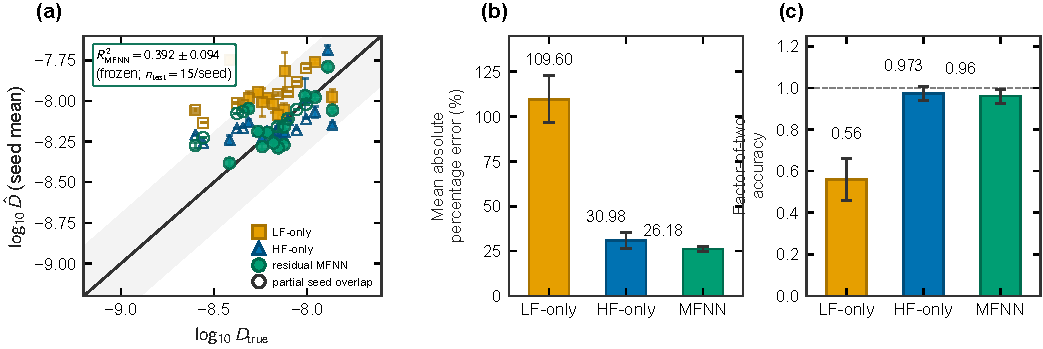
\includegraphics[width=\linewidth]{figures/Fig3_protocol_W_parity_metrics.pdf}
\caption{Protocol W (within-composition temperature hold-out; five seeds $0,1,2,42,123$; $n_{\mathrm{test}}=15$ per seed) for residual MFNN versus HF-only and LF-only. (a) Seed-mean $\log_{10}D$ parity with across-seed standard-deviation bars and a $\pm\log_{10}2$ (factor-of-two) band; filled markers denote samples present in all five seed test sets, open markers denote partial seed overlap. (b) MAPE (\%) and (c) Factor2 use frozen Table~\ref{tab:protocolW} values (MFNN MAPE $26.18\pm 1.33\,\%$; Factor2 $0.96\pm 0.033$) and are not recomputed from the scatter.}
\label{fig:protocolW}
\end{figure}

\begin{figure}[t]
\centering
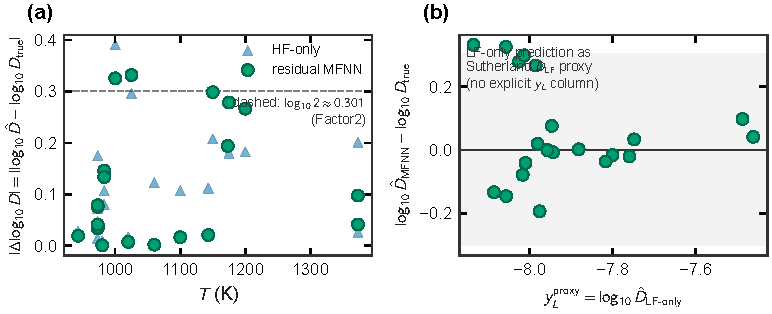
\includegraphics[width=\linewidth]{figures/Fig4_protocol_W_residual_topology.pdf}
\caption{Protocol W residual topology for the residual MFNN (seed-mean predictions over seeds containing each sample\_id).
(a) Absolute $\log_{10}D$ error versus temperature; dashed line: $\log_{10}2$ (Factor-of-two threshold); HF-only shown for context.
(b) Signed residual versus LF prior proxy ^{\mathrm{proxy}}=\log_{10}\hat{D}_{\mathrm{LF\text{-}only}}$ (prediction CSVs lack an explicit Sutherland {\mathrm{LF}}$ column); shaded band $\pm\log_{10}2$.
Does not alter frozen Protocol W metrics.}
\label{fig:residuals}
\end{figure}

\begin{figure}[t]
\centering
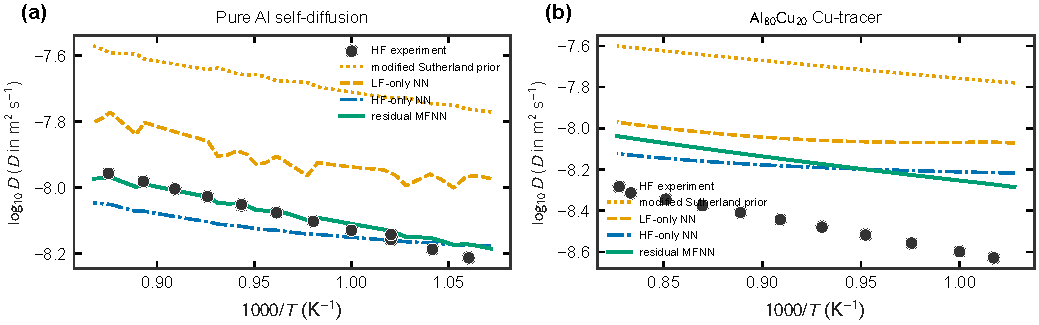
\includegraphics[width=\linewidth]{figures/Fig5_arrhenius_representative.pdf}
\caption{Representative Arrhenius-style $\log_{10}D$ vs $1000/T$ using Protocol W seed-42 weights (inference only; no retraining). (a) Pure Al self-diffusion; (b) $\mathrm{Al}_{80}\mathrm{Cu}_{20}$ Cu-tracer. Curves: residual MFNN, HF-only, LF-only, and modified Sutherland prior with honest $\eta(T)$. Not a LOGO success claim}
\label{fig:arrhenius}
\end{figure}


\subsection{Effect of resolving tracer vs interdiffusion labels (Al80Cu20)}
\label{sec:al80}

Before stratification by diffusion type, leave-one-group-out of mixed $\mathrm{Al}_{80}\mathrm{Cu}_{20}$ fails for label-semantic rather than purely compositional reasons. At nearly the same temperature, Cu-tracer diffusivities (Zhang et al.~\cite{zhang2010prl}; $\sim 2.3$--$4.9\times 10^{-9}\,\mathrm{m}^{2}\,\mathrm{s}^{-1}$) conflict with interdiffusivities ($\sim 7$--$8.9\times 10^{-9}\,\mathrm{m}^{2}\,\mathrm{s}^{-1}$) by a factor of approximately three, while the feature vector originally omitted diffusion type and training neighbors at nearby $x_{\mathrm{Cu}}$ remain inter-dominated. Viscosity pairing follows Schick et al.~\cite{schick2012}; missing $\eta$ rows are dropped, and no Kozlov-type silent fill of high-fidelity viscosity is employed.

After partitioning by diffusion type (still without a one-hot type feature), LOGO on the subgroups yields MFNN MAPE $\sim$28.8\% with Factor2 $=1$ for the interdiffusivity hold-out ($n=2$), versus MAPE $\sim$203\% with Factor2 $=0$ for the tracer hold-out ($n=10$). The mixed-group failure therefore concentrates on the dense Zhang tracer grid; interdiffusivity points at the same composition are comparatively well predicted once both scales are no longer forced onto a single scalar head (Fig.~\ref{fig:al80}). Under the one-hot setting of Sec.~\ref{sec:logo}, the stratified $\mathrm{Al}_{80}\mathrm{Cu}_{20}$ folds reach MAPE $6.48\%$ (Factor2 $=1$, $n=2$) for interdiffusivity and MAPE $156.49\%$ (Factor2 $=0$, $n=10$) for tracer.

\begin{figure}[t]
\centering
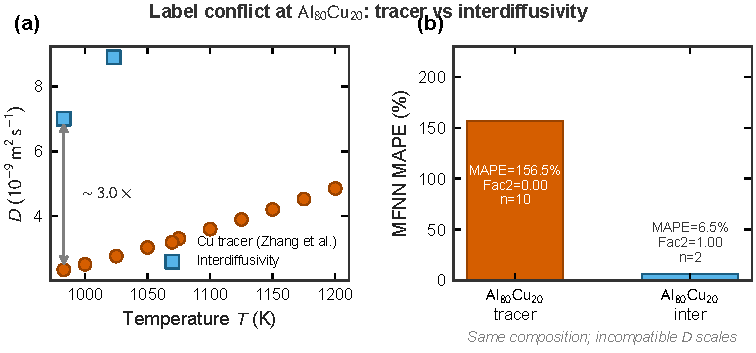
\includegraphics[width=\linewidth]{figures/Fig6_Al80_tracer_inter.pdf}
\caption{Label conflict at composition $\mathrm{Al}_{80}\mathrm{Cu}_{20}$. (a) High-fidelity diffusivity versus temperature: Cu-tracer data (Zhang et al.; open circles) lie systematically below interdiffusivity points (squares) by a factor of $\sim 3$ near $983\,\mathrm{K}$ ($D_{\mathrm{tracer}}\approx 2.35\times 10^{-9}$ vs $D_{\mathrm{inter}}\approx 7.0\times 10^{-9}\,\mathrm{m}^{2}\,\mathrm{s}^{-1}$). Without a \texttt{diff\_type} feature or group split, a single \texttt{comp\_group} cannot fit both scales. (b) Leave-one-group-out (LOGO) MFNN MAPE after splitting groups by \texttt{diff\_type} and adding a one-hot type feature: \texttt{Al80Cu20\_tracer} remains difficult (MAPE $156.5\,\%$, Factor2 $=0$, $n=10$), whereas \texttt{Al80Cu20\_inter} recovers (MAPE $6.5\,\%$, Factor2 $=1$, $n=2$).}
\label{fig:al80}
\end{figure}


\subsection{Leave-one-composition-out on Al--Cu}
\label{sec:logo}

Without a diffusion-type one-hot (12 features; 13 folds after subgrouping), MFNN MAPE is $44.11\pm 48.48\%$ across Al--Cu LOGO folds, with large variance driven by hard tracer hold-outs. With diffusion-type one-hot features (16 features; 13 folds), overall MAPE improves to $39.43\pm 39.71\%$. Stratified $\mathrm{Al}_{80}\mathrm{Cu}_{20}$ hold-outs under the one-hot setting are:

\begin{center}
\begin{tabular}{@{}lccc@{}}
\toprule
Hold-out & MFNN MAPE (\%) & Factor2 & $n$ \\
\midrule
Al80Cu20\_inter  & 6.48  & 1.0 & 2 \\
Al80Cu20\_tracer & 156.49 & 0.0 & 10 \\
\bottomrule
\end{tabular}
\end{center}

One-hot encoding improves the interdiffusivity fold and reduces overall LOGO MAPE, but does not recover the tracer fold when neighboring high-fidelity labels remain mostly inter-scale. Table~
ef{tab:logo} and Fig.~
ef{fig:logo} summarize the comparison. LOGO results are reported as Al--Cu--internal composition transfer only and are presented as a cautionary check rather than a headline claim.

\begin{table}[t]
\centering
\caption{Al--Cu leave-one-composition-out (LOGO) performance of MFNN. Population mean $\pm$ standard deviation over folds where applicable; stratified Al80Cu20 notes refer to the same fold set.}
\label{tab:logo}
\begin{tabular}{@{}llcl@{}}
\toprule
Configuration & Folds & MFNN MAPE (\%) & Notes \\
\midrule
Split by \texttt{diff\_type}, 12 feats
  & 13 & $44.11 \pm 48.48$
  & Al80\_inter $\sim$28.8\% (Fac2$=$1); Al80\_tracer $\sim$203\% (Fac2$=$0) \\
Split + \texttt{diff\_type} one-hot (16 feats)
  & 13 & $39.43 \pm 39.71$
  & Al80\_inter 6.48\% (Fac2$=$1); Al80\_tracer 156.49\% (Fac2$=$0) \\
\bottomrule
\end{tabular}
\end{table}

\begin{figure}[t]
\centering
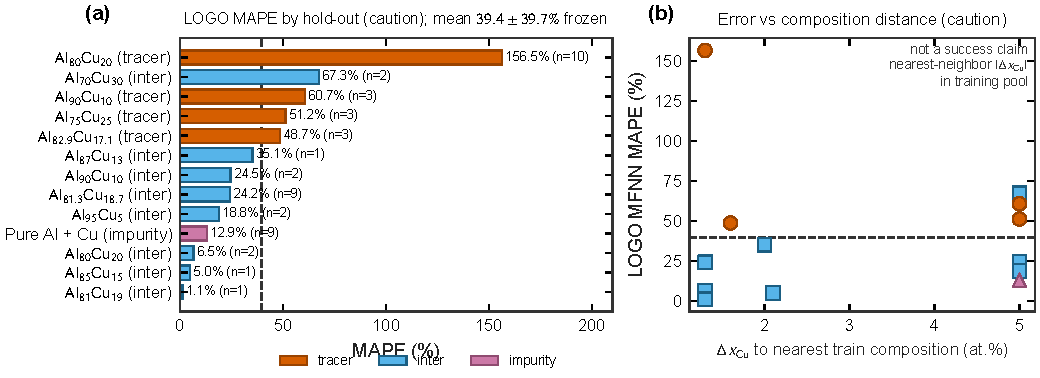
\includegraphics[width=\linewidth]{figures/Fig7_LOGO_distance_caution.pdf}
\caption{Al--Cu leave-one-group-out MFNN MAPE for each hold-out \texttt{comp\_group} after \texttt{diff\_type} splitting and one-hot features (13 folds; seed $42$). Bars are coloured by diffusivity type (tracer / inter / impurity). Annotations give the number of test points $n$ and Factor-of-two accuracy. The dashed line marks the unweighted mean MAPE across folds ($39.4\pm 39.7\,\%$). Extremes at \texttt{Al80Cu20\_tracer} (worst) and the recovered \texttt{Al80Cu20\_inter} fold are indicated. (a) MAPE by hold-out; (b) MAPE versus $\Delta x_{\mathrm{Cu}}$ to the nearest distinct HF training composition. Composition-extrapolation \textbf{caution} within Al--Cu only---not a headline success claim and not a cross-alloy-system transfer result.}
\label{fig:logo}
\end{figure}


\subsection{Ablation: separate tracer / inter models}
\label{sec:ablation}

Training separate networks on tracer-only and inter-only pools does not outperform the joint residual MFNN with a diffusion-type one-hot (Fig.~S5): Al80 tracer MAPE remains $\sim$173\% and Al80 inter $\sim$11\%. The tracer pool is sparse in neighboring compositions with honestly paired $\eta$; the inter pool can lack usable LF targets in some folds. An inter-only LOGO subset that excludes a pathological Al70Cu30 fold yields a more stable $\sim$18$\pm$17\% MAPE and is retained only as a sensitivity check. Separate training is therefore a negative ablation: the bottleneck is neighborhood sparsity of tracer high-fidelity labels under honest viscosity pairing, not the joint residual architecture.


\subsection{Random between-group protocol (caution)}
\label{sec:protocolG}

Protocol~G (random between-group splits, same five seeds; Fig.~S2) yields MFNN MAPE $27.36\pm 12.88\%$ and Factor2 $0.791\pm 0.257$. All seed hold-outs in this suite are Al--Cu groups, so seed-to-seed variance is dominated by which compositions enter the test set. Single-seed MAPE near $\sim$20\% is therefore not interpreted as final extrapolation performance. Protocol~G is reported strictly as a cautionary check in the Supplementary Information; the primary quantitative claim remains Protocol~W.


%% ============================================================

%% ============================================================

\section{Discussion}
\label{sec:discussion}

\subsection{Physics-guided residual correction under Protocol W}

Under Protocol~W, residual multi-fidelity correction improves mean accuracy and seed stability relative to HF-only (Table~\ref{tab:protocolW}; Figs.~\ref{fig:protocolW}--\ref{fig:arrhenius}). In sparse liquid-metal diffusivity regimes, single-fidelity networks are sensitive to weight initialization. The LF-only network $F_{\mathrm{L}}$---trained on Sutherland-generated $\log_{10} D_{\mathrm{LF}}$ from the modified Chen/Tang map~\cite{chen2014,tang2015}---carries large magnitude offsets from idealized Stokes--Einstein / Sutherland assumptions~\cite{sutherland1905,demmel2018}, yet it encodes the expected monotonic $\log_{10} D$--$T$ topology set by melt viscosity $\eta(T)$. Anchoring the predictor to that continuous LF manifold and learning only a smooth residual therefore acts as a physics-guided regularizer~\cite{willard2022,lu2020pnas,meng2020jcp,peherstorfer2018}: initialization variance shrinks without discarding the prior. Scientific content enters through the LF diffusivity channel (Sec.~\ref{sec:intro}), not through a governing-equation residual loss.

\subsection{Thermodynamic and neighborhood limits on composition transfer}

Al--Cu leave-one-composition-out is limited by label semantics and neighborhood structure rather than $x_{\mathrm{Cu}}$ distance alone. Mixed $\mathrm{Al}_{80}\mathrm{Cu}_{20}$ juxtaposes Cu-tracer and interdiffusivity high-fidelity labels at nearly the same temperature (Sec.~\ref{sec:al80}; Fig.~\ref{fig:al80}); after subgrouping and one-hot encoding, interdiffusivity folds become tractable while the tracer fold remains failed because nearby training neighbors are inter-dominated (Table~\ref{tab:logo}; Fig.~\ref{fig:logo}). Separate tracer/inter networks do not outperform the joint residual MFNN with one-hot features (Fig.~S5). These LOGO results are Al--Cu--internal cautionary checks, not evidence of robust cross-composition or cross-system generalization.

\subsection{Counterfactual slope--intercept diagnostics (SI only)}


Oracle checks that access held-out composition labels separate Arrhenius slope error from thermodynamic scale error on the failed Al80Cu20 tracer fold; they are not valid evaluation protocols. A post-hoc logarithmic offset at \,\mathrm{K}$ ($\delta = -0.482\pm 0.046\approx -\log_{10} 3$) cuts residual MAPE on the remaining temperatures from .20\pm 28.78\%$ to .81\pm 1.73\%$ (Factor2 \to 1$; Fig.~S4), whereas unweighted re-inclusion of that anchor leaves MAPE near $\sim\%. Endpoint-anchor upweighting ({=}2$, =1\to 5\to 10$) lowers MAPE from \%$ to \%$ to \%$ (Fig.~S6). The LF channel already captures the temperature slope; LOGO failure tracks an unmodeled $\sim 3\times$ tracer--inter scale offset (missing Darken factor $\Phi$~\cite{Darken1948}) plus dilution of sparse tracer anchors under unweighted MSE. These diagnostics explain mechanism only and do not replace Protocol~W.

\subsection{Methodological scope and outlook}

The primary quantitative claim remains Protocol~W ($n_{\mathrm{test}}=15$). Protocol~G and Al--Cu LOGO are cautionary; detailed claim-boundary items are collected in Sec.~\ref{sec:limitations}. Progress on tracer LOGO requires more $\eta$-paired tracer high-fidelity points at neighboring compositions. A Darken-type $\Phi$~\cite{Darken1948} is a natural next step for the diagnosed scale mismatch without changing the residual MFNN architecture or Protocol~W claims; coupling to CALPHAD / DICTRA-type workflows~\cite{andersson2002,tang2015} remains a longer-term target once tracer neighborhoods thicken.

\section{Limitations}
\label{sec:limitations}

\begin{itemize}
\item \textbf{Primary claim scope.} Protocol W measures within-composition temperature generalization ($n_{\mathrm{test}}=15$). It is not composition leave-out and must not be paraphrased as LOGO success.

\item \textbf{Protocol G is cautionary.} Random between-group MFNN MAPE $27.4\pm 12.9\%$ has large seed variance; low single-seed values are not final extrapolation performance and are not headline results.

\item \textbf{LOGO is Al--Cu--internal only.} Overall split + one-hot LOGO MAPE $\sim 39.4\pm 39.7\%$ coexists with Al80\_inter success (6.48\%, Factor2 $= 1$) and Al80\_tracer failure ($\sim$156\%, Factor2 $= 0$). No cross-system LOGO is claimed.

\item \textbf{\texttt{diff\_type} semantics.} Tracer and interdiffusivity labels are not interchangeable; one-hot encoding helps inter folds but does not rescue dense tracer grids when neighbors are inter-scale.

\item \textbf{Separate models.} Tracer-only / inter-only training did not beat joint MFNN + \texttt{diff\_type} one-hot; architecture splitting is not a remedy for sparse tracer neighborhoods.

\item \textbf{Viscosity honesty.} Missing $\eta$ rows are dropped. Kozlov alloy viscosity is never used as silent HF $\eta$. Assael / Schick-class sources~\cite{assael2006,schick2012} are preferred where applicable.

\item \textbf{Densified Arrhenius samples.} Zhang (and related) temperature-grid points from Arrhenius parameters~\cite{zhang2010prl} are densified samples, not independent experiments; effective experimental diversity is lower than raw row counts suggest.

\item \textbf{System coverage.} The usable table is Al--Cu--dominated. Al--Mg--Si and Al--Ce--Ni coverage is insufficient for system-level or cross-system leave-one-out claims.

\item \textbf{Moderate $R^{2}$.} Protocol W $R^{2}=0.392\pm 0.094$ on $\log_{10} D$ reflects a small heterogeneous test pool; Factor2 and MAPE remain the primary reported metrics.

\item \textbf{Scope relative to Meng/Lu.} Residual / composite multi-fidelity regression~\cite{lu2020pnas,meng2020jcp} for $\eta\to D$ only (not a PDE-residual PINN/PPINN; Sec.~\ref{sec:intro}).
\end{itemize}

%% ============================================================
\section{Conclusions}
\label{sec:conclusions}

A residual multi-fidelity network that corrects a Sutherland-type $\eta\to D$ prior toward experimental diffusivities yields improved, more stable within-composition temperature generalization for Al-dominated melt data (protocol W: MFNN MAPE $26.18\pm 1.33\%$, Factor2 $0.96\pm 0.033$ over five seeds), outperforming HF-only and LF-only baselines under honest viscosity pairing. Composition leave-out on Al--Cu remains constrained by tracer versus interdiffusivity label structure and by sparse tracer HF neighborhoods; random between-group splits are likewise too seed-sensitive for headline use. Future gains depend less on changing the residual MFNN form than on expanding tracer HF tables with measured $\eta$ at neighboring compositions and on keeping diffusion-type semantics explicit in both data and evaluation.

%% ============================================================
\section*{Data availability}

Curated diffusivity--viscosity tables, evaluation fold definitions, training/evaluation scripts, and aggregated metrics underlying Tables~\ref{tab:protocolW} and~\ref{tab:logo} (and SI $\alpha$ table) are openly available at \url{https://github.com/JunHuaBai96/mfnn_eta_to_D}. Main-text figure sources correspond to Figs.~\ref{fig:mfnn}--\ref{fig:logo} (seven main figures, Figs.~1--7, including Protocol~W panel~(c)). The oracle diagnostic Fig.~S4 is maintained with the manuscript submission package and in the same repository.

\section*{Code availability}

Training and evaluation scripts (Adam$\to$L-BFGS residual MFNN; protocols W / G / LOGO; seeds $\{0,1,2,42,123\}$; targets $\log_{10} D$; no Kozlov silent HF $\eta$) are openly available at \url{https://github.com/JunHuaBai96/mfnn_eta_to_D}.


% --- Strict Gemini SI figures S1-S5 (paths under figures/) ---
% FigS1_alpha_mixing_weights.pdf
% FigS2_protocol_G_variance.pdf
% FigS3_al80_anchor_k.pdf
% FigS4_al80_posthoc_shift.pdf
% FigS5_difftype_split_ablation.pdf
% Optional: FigS6_al80_upweight_w.pdf
\bibliographystyle{elsarticle-num}
\bibliography{refs}

\end{document}
